% 2009 年福建卷文科第 22 题：椭圆 x^2/4+y^2=1、直线 l:x=10/3 与点 A、B、S、M、N。
% 来源 PDF：普通高考/2009/2009福建文.pdf，SHA-256 f0a5111a6f86f4d4e8618c5c2cd0ecfd678a590b36ecbd033bb63b189700a0bc。
% 原页：第 2 页（A3 三栏）第 3 栏上部，书页码 518。
% 重绘依据：取 |MN| 最小时的 S(6/5,4/5)，M(10/3,4/3)、N(10/3,-4/3)。
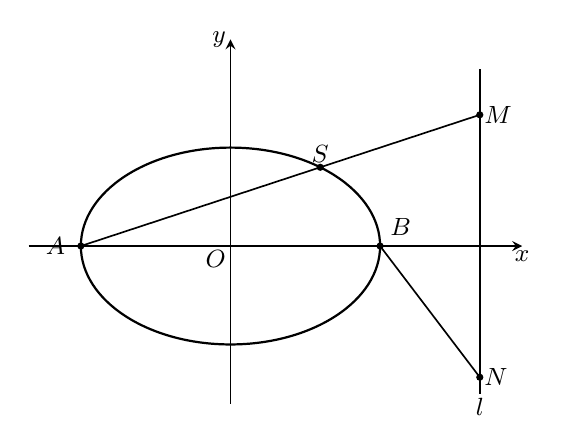
\begin{tikzpicture}[semithick, x=0.95cm, y=1.25cm, every node/.style={inner sep=1.4pt, font=\small}]
  % 坐标轴
  \draw[-stealth] (-2.7,0) -- (3.9,0) node[below] {$x$};
  \draw[-stealth] (0,-1.6) -- (0,2.1) node[left] {$y$};
  \node[below left] at (0,0) {$O$};

  % 椭圆
  \draw[thick] (0,0) ellipse (2 and 1);

  % 直线 l
  \draw (3.333,-1.5) -- (3.333,1.8);
  \node[below] at (3.333,-1.5) {$l$};

  % 点
  \coordinate (A) at (-2,0);
  \coordinate (B) at (2,0);
  \coordinate (S) at (1.2,0.8);
  \coordinate (M) at (3.333,1.333);
  \coordinate (N) at (3.333,-1.333);
  \fill (A) circle (1.3pt);
  \fill (B) circle (1.3pt);
  \fill (S) circle (1.3pt);
  \fill (M) circle (1.3pt);
  \fill (N) circle (1.3pt);

  % 直线
  \draw (A) -- (M);
  \draw (B) -- (N);

  % 标注
  \node[left=4pt] at (A) {$A$};
  \node[above right=2pt] at (B) {$B$};
  \node[above] at (S) {$S$};
  \node[right] at (M) {$M$};
  \node[right] at (N) {$N$};
\end{tikzpicture}
